\chapter{Evaluation}

\section{Customer Requirements}

For this section I will be evaluating whether or not my system has met my initial objectives that were proposed in the Analysis section. This will be used to determine whether or not the system has met the customer requirements. If the system does not meet an objective then I will include a further explanation of why this is the case. If the objective has been met then I will provide evidence to support this evaluation.

The objectives have been split into:
\begin{itemize}
\item{General Objectives}
\item{Specific Objectives}
\item{Core Objectives}
\item{Other Objectives}
\end{itemize}

%include as many subsections as necessary for your objectives
\paragraph{General Objectives}

\subsection{Database Functionality}

\textbf{Objective:} A database to show all current staff (with details such as their job title) and the hardware devices they are assigned to.

\textbf{Has the objective been fulfilled?}

This objective has been fulfilled. I have met this objective by examining the company's current spreadsheet (their current way to store data) and making sure that all the correct fields were included in my database. To display allocation of hardware devices to staff members it was important to make the database relational, this was done with the use of primary and foreign keys. Using this method means hardware can be added to a separate table to staff and then linked in the StaffHardware table which the staff members will see.

\textbf{Evidence}

Below are the different interfaces that will present the database that shows current staff and their assigned hardware devices.

\begin{figure}[H]
    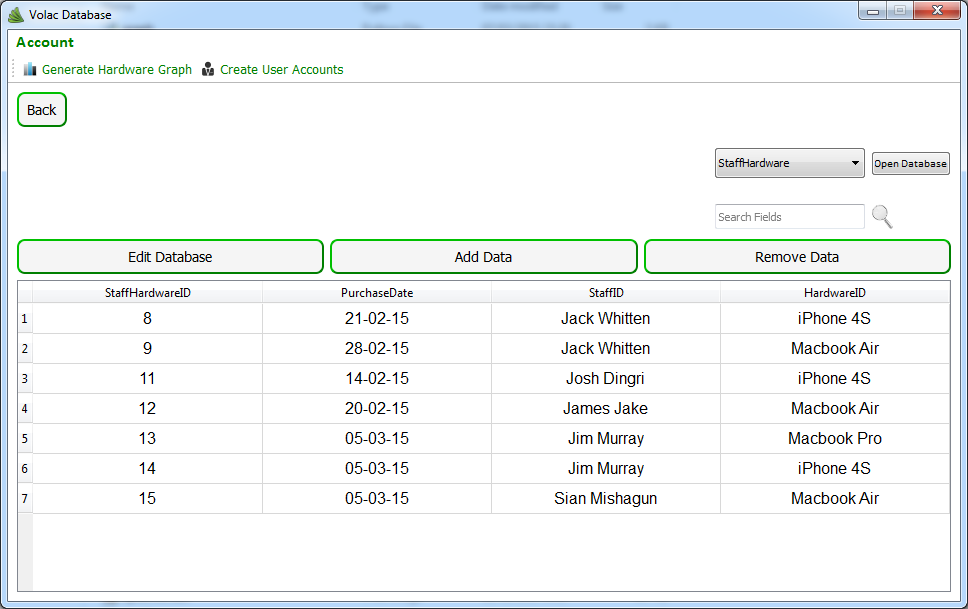
\includegraphics[width=\textwidth]{./Evaluation/Images/Database1.png}
    \caption{The Admin interface, viewing the StaffHardware Table.} \label{fig:db1}
\end{figure}

\begin{figure}[H]
    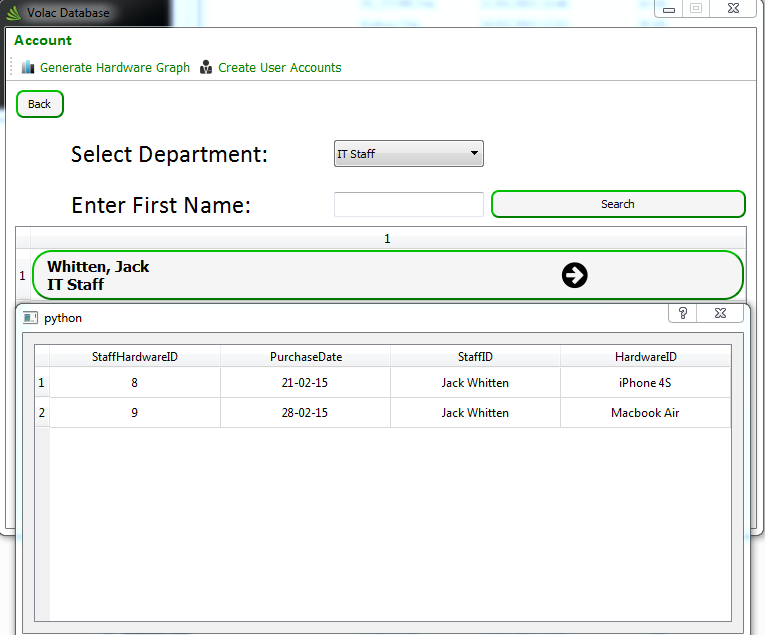
\includegraphics[width=\textwidth]{./Evaluation/Images/database3.png}
    \caption{The Admin interface: When searching for data and clicking to view more information, the StaffHardware table will appear.} \label{fig:db2}
\end{figure}

\begin{figure}[H]
    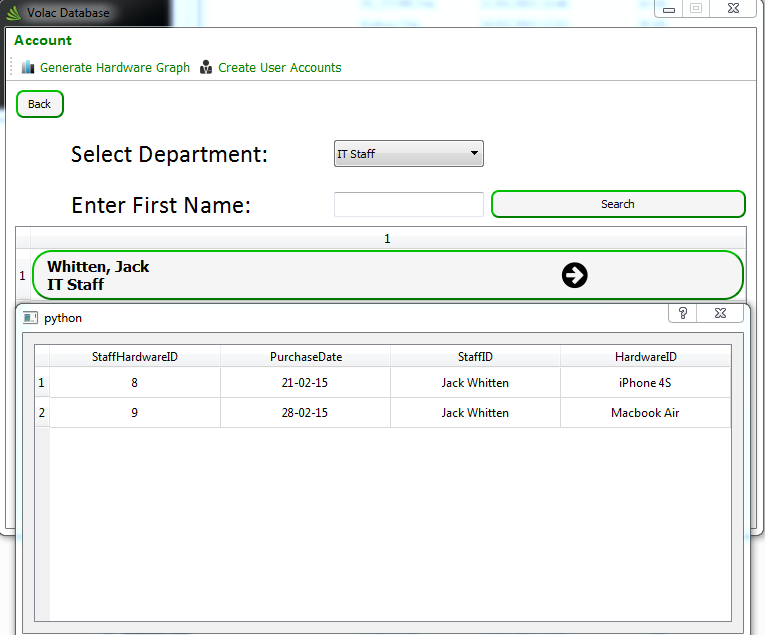
\includegraphics[width=\textwidth]{./Evaluation/Images/database3.png}
    \caption{The Manager (and staff) interface, viewing their current hardware devices.} \label{fig:db3}
\end{figure}

\subsection{Clear Database Structure}

\textbf{Objective:} The database will replace the current spreadsheet and be easy to read as information will be clear and organized.

\textbf{Has the objective been fulfilled?}

\textbf{Evidence}


\subsection{Easy to use Data Input and Keyboard Shortcuts}

\textbf{Objective:} An easy to use database for IT staff to enter colleague data with toolbar buttons and keyboard shortcuts as they are advanced computer users and will want an quicker way of doing things.

\textbf{Has the objective been fulfilled?}

\textbf{Evidence}


\subsection{Simple Interface Structure}

\textbf{Objective:} The layout for colleagues to see their hardware allocations will be clear and to the point, missing out any unnecessary buttons and menus.

\textbf{Has the objective been fulfilled?}

\textbf{Evidence}


\subsection{Search Functionality}

\textbf{Objective:} A search function will be in place to make searching for a field (such as staff member or hardware device) easy.

\textbf{Has the objective been fulfilled?}

\textbf{Evidence}



%%%%
\paragraph{Specific Objectives}

\subsection{Tables}

\textbf{Objective:}The database will have one table with staff and a relationship to the table with their hardware device. This will show which hardware devices the staff are allocated and all the details of that hardware device. Staff details including department and location will be linked to the Department and Location tables.

\textbf{Has the objective been fulfilled?}

\textbf{Evidence}



\subsection{---}

\textbf{Objective:}The search function will allow a user to enter text and will highlight where on the page that text is.

\textbf{Has the objective been fulfilled?}

\textbf{Evidence}



\subsection{--}

\textbf{Objective:} Read-Only access for staff viewing their own information (with a log-in system to allow this).

\textbf{Has the objective been fulfilled?}

\textbf{Evidence}



\subsection{Tables}

\textbf{Objective:}Read-Only access for line managers wanting to see all data about staff in their department.

\textbf{Has the objective been fulfilled?}

\textbf{Evidence}



\subsection{--}

\textbf{Objective:}Admin rights for IT staff so they are able to view and edit all data on the database.

\textbf{Has the objective been fulfilled?}

\textbf{Evidence}



\subsection{--}

\textbf{Objective:}An automatic email will be sent to IT staff members reminding them that a warranty is running out on a particular device, this email will be sent about 3 months before the end of the warranty period.

\textbf{Has the objective been fulfilled?}

\textbf{Evidence}



\subsection{--}

\textbf{Objective:} Users will be able to query information, for example if they wanted to show only mobile phones or if they wanted to show only specific departments.

\textbf{Has the objective been fulfilled?}

\textbf{Evidence}



\subsection{--}

\textbf{Objective:}A method of sending hardware request forms electronically may be introduced to elimate the need for physical copies.

\textbf{Has the objective been fulfilled?}

\textbf{Evidence}


\subsection{--}

\textbf{Objective:}The database may be online using the company's server, this will mean that users will be able to access the database from anywhere.

\textbf{Has the objective been fulfilled?}

\textbf{Evidence}


\paragraph{Core Objectives}

\subsection{--}

\textbf{Objective:}The system will provide a login system where IT staff can assign usernames to all staff and have admin rights to view all data. The database will have read-only access for colleagues viewing their own information. Managers will be able to view their departments hardware devices.

\textbf{Has the objective been fulfilled?}

\textbf{Evidence}

\subsection{--}

\textbf{Objective:}The system will also have an automatic email sent to IT staff members reminding them that a warranty is running out on a particular device, this email will be sent about 3 months before the end of the warranty period.

\textbf{Has the objective been fulfilled?}

\textbf{Evidence}

\subsection{--}

\textbf{Objective:}The system must have a search function to allow a user to find a specific field.

\textbf{Has the objective been fulfilled?}

\textbf{Evidence}

\subsection{--}

\textbf{Objective:}The system must have a way to query information so that a user can filter or catergorise information (such as by department or location)

\textbf{Has the objective been fulfilled?}

\textbf{Evidence}


\paragraph{Other Objectives}

\subsection{--}

\textbf{Objective:}It will be nice to include a method of sending hardware request forms electronically to elimate the need for physical copies. However this will only be considered if everything else is completed as it is not essential.

\textbf{Has the objective been fulfilled?}

\textbf{Evidence}

\subsection{--}

\textbf{Objective:}A great feature to have is the database being available online using the server the company owns. If the database was online it will be available to use from anywhere with internet connection.

\textbf{Has the objective been fulfilled?}

\textbf{Evidence}





\section{Effectiveness}

%include as many subsections as necessary for your objectives
\subsection{Objective Evaluation}

\section{Learnability}

\section{Usability}

\section{Maintainability}

\section{Suggestions for Improvement}

\section{End User Evidence}

\subsection{Questionnaires}

\subsection{Graphs}

\subsection{Written Statements}
